\documentclass[class=article, crop=false]{standalone}
\usepackage{my_preamble}
\begin{document}
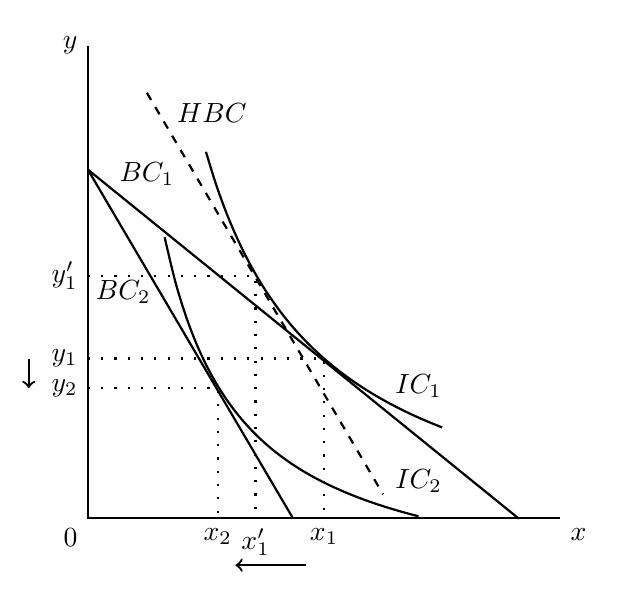
\begin{tikzpicture}[thick,font=\sffamily,scale=1.5]
	%axis
	\draw (0,4) node[left]{$y$} -- (0,0) node[below left] {$0$} -- (4,0) node[below right]{$x$}; %labels
	
	%curves
	\draw plot[domain=0:3.65,smooth] (\x,2.95-0.81*\x); %BC1
	\draw plot[domain=0:1.73,smooth] (\x,2.95-1.7*\x); %BC2
	\draw plot[domain=1:3,smooth] (\x,3.5/\x-0.4); %IC1
	\draw plot[domain=0.65:2.8,smooth] (\x,2/\x-0.7); %IC2

	%dotted lines
	\draw[loosely dotted] (0,1.35) node[left]{$y_1$} -| node[pos=0.25,below=3mm] {} (2,0) node[below]{$x_1$}; %dotted lines 1
	\draw[loosely dotted] (0,1.1) node[left]{$y_2$} -| node[pos=0.25,below=3mm] {} (1.1,0) node[below]{$x_2$}; %dotted lines 2
	
	%labels and arrows
	\node[below] at (0.5,3.1) {$BC_{1}$}; %BC1 label
	\node[below] at (0.3,2.1) {$BC_{2}$}; %BC2 label
	\node[below] at (2.8,1.3) {$IC_{1}$}; %IC1 label
	\node[below] at (2.8,0.5) {$IC_{2}$}; %IC2 label
	\draw [->] (1.85,-0.4) -- (1.25,-0.4); %x arrow
	\draw [->] (-0.5,1.35) -- (-0.5,1.1); %y arrow

	%Hypothetical
	\draw [dashed] plot[domain=0.5:2.5] (\x,4.45-1.7*\x); %BC2
	\node[below] at (1.05,3.6) {$HBC$}; %HBC label

	%CV
	\draw[loosely dotted] (0,2.05) node[left]{$y^\prime_1$} -| node[pos=0.25,below=3mm] {} (1.42,0) node[below]{$x^\prime_1$}; %dotted lines
\end{tikzpicture}
\end{document}